\documentclass[11pt]{article}
\usepackage[T1,T2A]{fontenc}
\usepackage[utf8]{inputenc}
\usepackage[english,russian]{babel}
\usepackage{graphicx}
\usepackage{amsmath}
\graphicspath {{img/}}

\title{\textbf{Лабораторная работа №5\\<<Исследование устройств частотного преобразования сигналов в системах передачи информации>>}}
\author{Перепелица А.А., ККСО-01-19}
\date{Москва, 2022 г.}
\addtolength{\topmargin}{-3cm}
\addtolength{\textheight}{3cm}
\begin{document}
\maketitle
\thispagestyle{empty}
\textbf{Цель работы:} ознакомление с устройством, работой фазовых модуляторов и демодуляторов сигналов, и приобретение практических навыков  моделирования этих устройств. 

\section{Схема №1: исследование ФМ сигналов}
\subsection{Перечень элементов, использованных в схемах, с
их краткими характеристиками}
\begin{itemize}
    \item[-] Источник переменного тока (1 В, 10 кГц, $0^\circ$)
    \item[-] 4-канальный осциллограф
    \item[-] Источник напряжения частотной модуляции (1 В/В, 0 В)
    \item[-] Анализатор спектра
    \item[-] Генератор сигналов 
\end{itemize}


\subsection{Копии окон схемных файлов с позиционными обозначениями}
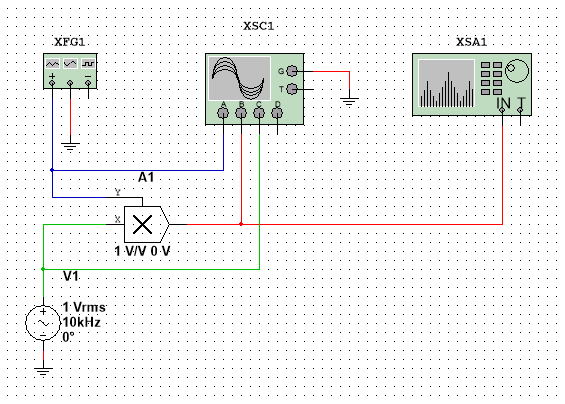
\includegraphics[width=1\linewidth]{img/scheme1.png}
\begin{center}
    Рис.1 Схема исследования ФМ сигналов
\end{center}


\subsection{Результаты расчетов и измерений приборами}
\begin{center}
    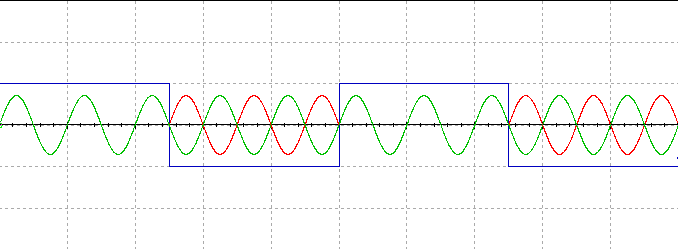
\includegraphics[width=1\linewidth]{img/osc1.png}
        Рис.2 Показания осциллографа.
\end{center}

\begin{center}
    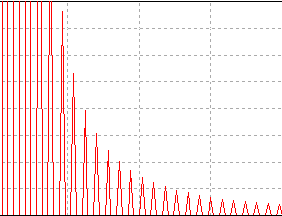
\includegraphics[width=1\linewidth]{img/chast1.png}
        Рис.3 Показания анализатора спектра.
\end{center}


\newpage
\section{Схема №2: Схема частотного модулятора и демодулятора}
\subsection{Перечень элементов, использованных в схемах, с их краткими характеристиками}
\begin{itemize}
    \item[-] 4-канальный осциллограф
    \item[-] Генератор сигналов
    \item[-] Источник переменного тока (1 В, 10 кГц, $0^\circ$)
    \item[-] Резистор (100 Ом)
    \item[-] Конденсатор (0.5 мкФ)
    \item[-] Резистор (100 Ом)
    \item[-] Множитель напряжения (1 В/В, 0 В), 2 шт.  
\end{itemize}

\subsection{Копии окон схемных файлов с позиционными обозначениями}
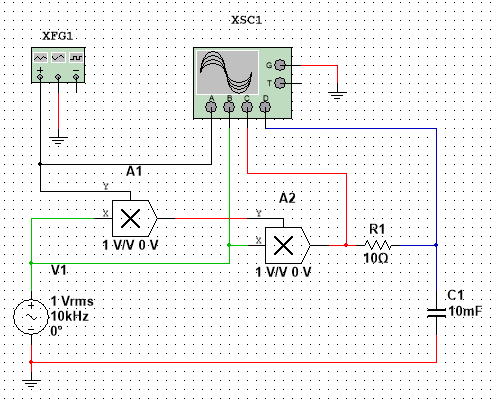
\includegraphics[width=1\linewidth]{img/scheme2.png}
\begin{center}
    Рис.4 Схема частотного модулятора и демодулятора
\end{center}

\subsection{Результаты расчетов и измерений приборами}
\begin{center}
    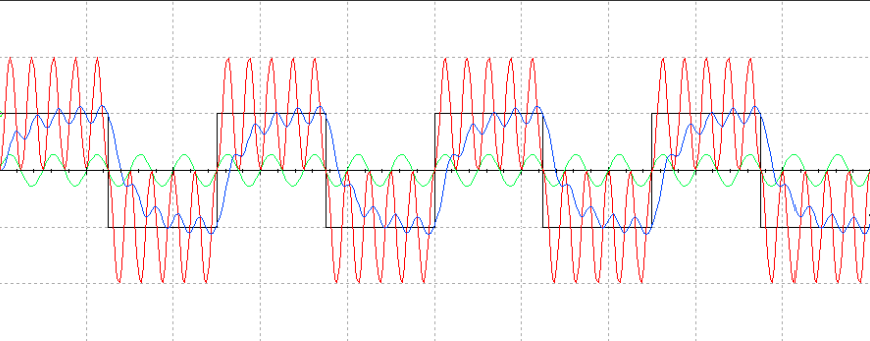
\includegraphics[width=1\linewidth]{img/osc2.png}
        Рис.5 Показания осциллографа.
\end{center}


\newpage
\section{Схема №3: Исследование модели системы передачи информации с фазовой манипуляцией}
\subsection{Перечень элементов, использованных в схемах, с
их краткими характеристиками}
\begin{itemize}
    \item[-] Генератор слов 
    \item[-] 4-канальный осциллограф
    \item[-] ЦАП
    \item[-] Источник постоянного тока (20 В)
    \item[-] Источник постоянного тока (5 В)
    \item[-] Источник переменного тока (1 В, 10 кГц, $0^\circ$)
    \item[-] Множитель напряжения (1 В/В, 0 В), 2 шт. 
    \item[-] Резистор (100 Ом) 3 шт.
    \item[-] Линия связи без потерь (100 Ом, 1 нС)
    \item[-] Конденсатор (0.3 мкФ)
    \item[-] Гистерезис по напряжению (0.2 В, 0.7В/В)
    \item[-] Логический анализатор
\end{itemize}


\subsection{Копии окон схемных файлов с позиционными обозначениями}
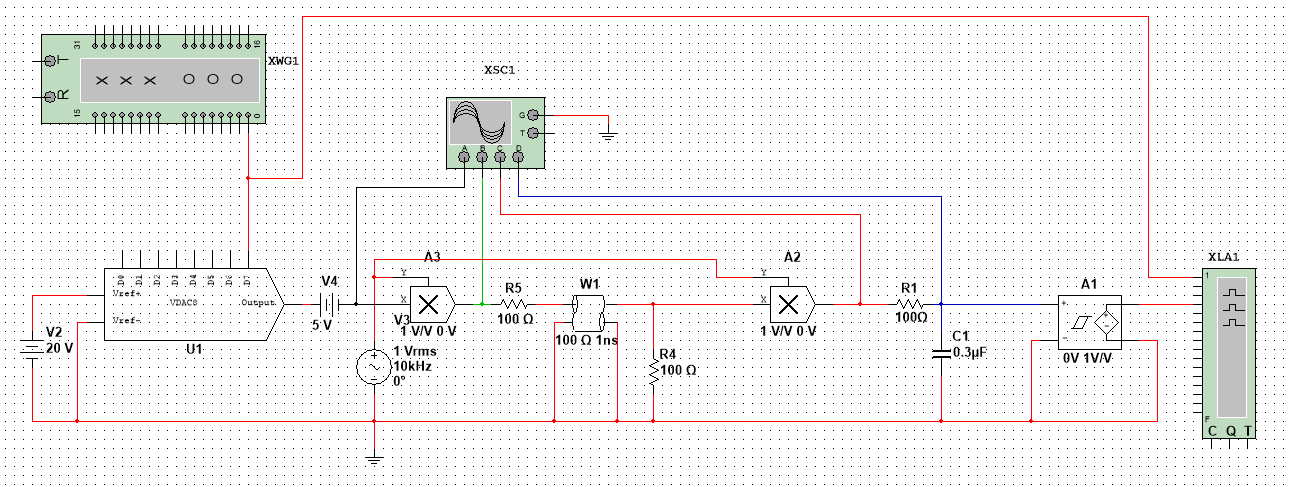
\includegraphics[width=1\linewidth]{img/scheme3.png}
\begin{center}
    Рис.7 Схема модели системы передачи информации с фазовой манипуляцией
\end{center}

\subsection{Результаты расчетов и измерений приборами}
Показания осциллографа будут различаться при разных скоростях передачи информации.
\begin{center}
    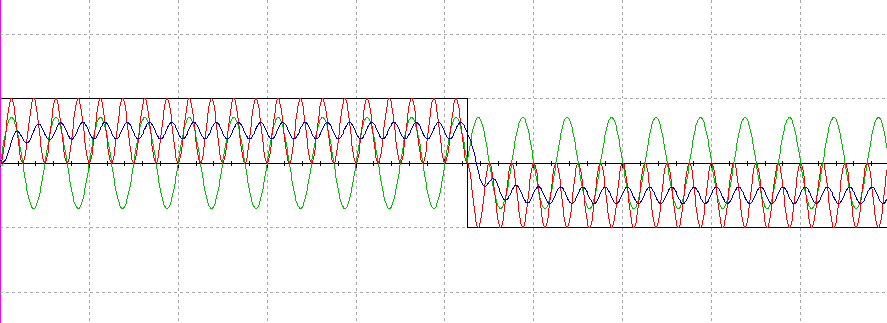
\includegraphics[width=1\linewidth]{img/osc31.png}
        Рис.8 Показания осциллографа при скорости передачи 1 Кбит/с.
\end{center}

\begin{center}
    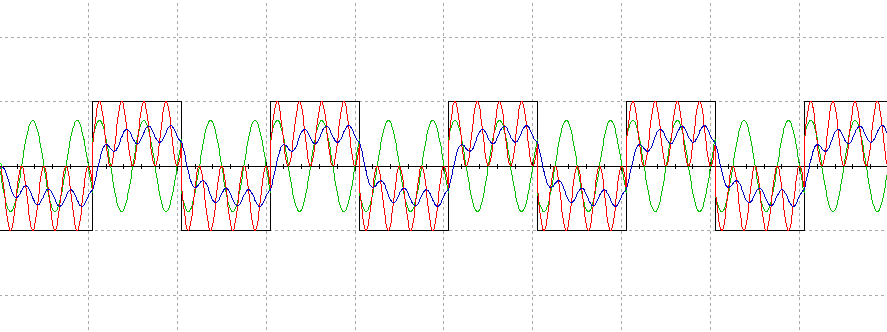
\includegraphics[width=1\linewidth]{img/osc32.png}
        Рис.9 Показания осциллографа при скорости передачи 5 Кбит/с.
\end{center}
\begin{center}
    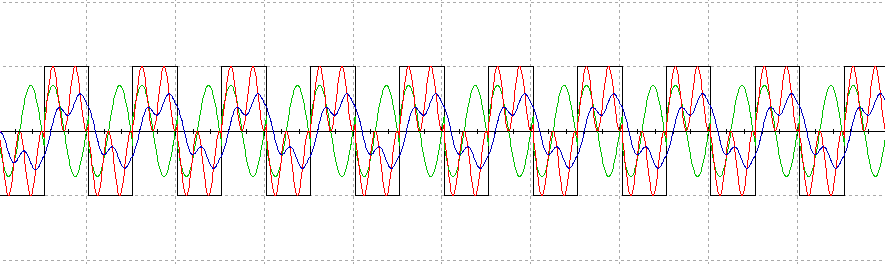
\includegraphics[width=1\linewidth]{img/osc33.png}
        Рис.10 Показания осциллографа при скорости передачи 10 Кбит/с.
\end{center}

\textbf{Вывод:} в ходе выполнения лабораторной работы мы изучили ,устройства фазового преобразования сигналов, и их работу, а также практические навыки, научились моделировать эти устройства.


\end{document}